\documentclass[twoside]{book}

% Packages required by doxygen
\usepackage{fixltx2e}
\usepackage{calc}
\usepackage{doxygen}
\usepackage[export]{adjustbox} % also loads graphicx
\usepackage{graphicx}
\usepackage[utf8]{inputenc}
\usepackage{makeidx}
\usepackage{multicol}
\usepackage{multirow}
\PassOptionsToPackage{warn}{textcomp}
\usepackage{textcomp}
\usepackage[nointegrals]{wasysym}
\usepackage[table]{xcolor}

% Font selection
\usepackage[T1]{fontenc}
\usepackage[scaled=.90]{helvet}
\usepackage{courier}
\usepackage{amssymb}
\usepackage{sectsty}
\renewcommand{\familydefault}{\sfdefault}
\allsectionsfont{%
  \fontseries{bc}\selectfont%
  \color{darkgray}%
}
\renewcommand{\DoxyLabelFont}{%
  \fontseries{bc}\selectfont%
  \color{darkgray}%
}
\newcommand{\+}{\discretionary{\mbox{\scriptsize$\hookleftarrow$}}{}{}}

% Page & text layout
\usepackage{geometry}
\geometry{%
  a4paper,%
  top=2.5cm,%
  bottom=2.5cm,%
  left=2.5cm,%
  right=2.5cm%
}
\tolerance=750
\hfuzz=15pt
\hbadness=750
\setlength{\emergencystretch}{15pt}
\setlength{\parindent}{0cm}
\setlength{\parskip}{3ex plus 2ex minus 2ex}
\makeatletter
\renewcommand{\paragraph}{%
  \@startsection{paragraph}{4}{0ex}{-1.0ex}{1.0ex}{%
    \normalfont\normalsize\bfseries\SS@parafont%
  }%
}
\renewcommand{\subparagraph}{%
  \@startsection{subparagraph}{5}{0ex}{-1.0ex}{1.0ex}{%
    \normalfont\normalsize\bfseries\SS@subparafont%
  }%
}
\makeatother

% Headers & footers
\usepackage{fancyhdr}
\pagestyle{fancyplain}
\fancyhead[LE]{\fancyplain{}{\bfseries\thepage}}
\fancyhead[CE]{\fancyplain{}{}}
\fancyhead[RE]{\fancyplain{}{\bfseries\leftmark}}
\fancyhead[LO]{\fancyplain{}{\bfseries\rightmark}}
\fancyhead[CO]{\fancyplain{}{}}
\fancyhead[RO]{\fancyplain{}{\bfseries\thepage}}
\fancyfoot[LE]{\fancyplain{}{}}
\fancyfoot[CE]{\fancyplain{}{}}
\fancyfoot[RE]{\fancyplain{}{\bfseries\scriptsize Generated by Doxygen }}
\fancyfoot[LO]{\fancyplain{}{\bfseries\scriptsize Generated by Doxygen }}
\fancyfoot[CO]{\fancyplain{}{}}
\fancyfoot[RO]{\fancyplain{}{}}
\renewcommand{\footrulewidth}{0.4pt}
\renewcommand{\chaptermark}[1]{%
  \markboth{#1}{}%
}
\renewcommand{\sectionmark}[1]{%
  \markright{\thesection\ #1}%
}

% Indices & bibliography
\usepackage{natbib}
\usepackage[titles]{tocloft}
\setcounter{tocdepth}{3}
\setcounter{secnumdepth}{5}
\makeindex

% Hyperlinks (required, but should be loaded last)
\usepackage{ifpdf}
\ifpdf
  \usepackage[pdftex,pagebackref=true]{hyperref}
\else
  \usepackage[ps2pdf,pagebackref=true]{hyperref}
\fi
\hypersetup{%
  colorlinks=true,%
  linkcolor=blue,%
  citecolor=blue,%
  unicode%
}

% Custom commands
\newcommand{\clearemptydoublepage}{%
  \newpage{\pagestyle{empty}\cleardoublepage}%
}

\usepackage{caption}
\captionsetup{labelsep=space,justification=centering,font={bf},singlelinecheck=off,skip=4pt,position=top}

%===== C O N T E N T S =====

\begin{document}

% Titlepage & ToC
\hypersetup{pageanchor=false,
             bookmarksnumbered=true,
             pdfencoding=unicode
            }
\pagenumbering{alph}
\begin{titlepage}
\vspace*{7cm}
\begin{center}%
{\Large My Project }\\
\vspace*{1cm}
{\large Generated by Doxygen 1.8.13}\\
\end{center}
\end{titlepage}
\clearemptydoublepage
\pagenumbering{roman}
\tableofcontents
\clearemptydoublepage
\pagenumbering{arabic}
\hypersetup{pageanchor=true}

%--- Begin generated contents ---
\chapter{Hierarchical Index}
\section{Class Hierarchy}
This inheritance list is sorted roughly, but not completely, alphabetically\+:\begin{DoxyCompactList}
\item \contentsline{section}{Board}{\pageref{class_board}}{}
\item \contentsline{section}{Game}{\pageref{class_game}}{}
\begin{DoxyCompactList}
\item \contentsline{section}{BT}{\pageref{class_b_t}}{}
\item \contentsline{section}{FaH}{\pageref{class_fa_h}}{}
\item \contentsline{section}{M\+BT}{\pageref{class_m_b_t}}{}
\end{DoxyCompactList}
\item \contentsline{section}{Piece}{\pageref{class_piece}}{}
\item \contentsline{section}{Player}{\pageref{class_player}}{}
\item \contentsline{section}{Position}{\pageref{struct_position}}{}
\end{DoxyCompactList}

\chapter{Class Index}
\section{Class List}
Here are the classes, structs, unions and interfaces with brief descriptions\+:\begin{DoxyCompactList}
\item\contentsline{section}{\hyperlink{class_board}{Board} }{\pageref{class_board}}{}
\item\contentsline{section}{\hyperlink{class_b_t}{BT} }{\pageref{class_b_t}}{}
\item\contentsline{section}{\hyperlink{class_fa_h}{FaH} }{\pageref{class_fa_h}}{}
\item\contentsline{section}{\hyperlink{class_game}{Game} }{\pageref{class_game}}{}
\item\contentsline{section}{\hyperlink{class_m_b_t}{M\+BT} }{\pageref{class_m_b_t}}{}
\item\contentsline{section}{\hyperlink{class_piece}{Piece} }{\pageref{class_piece}}{}
\item\contentsline{section}{\hyperlink{class_player}{Player} }{\pageref{class_player}}{}
\item\contentsline{section}{\hyperlink{struct_position}{Position} }{\pageref{struct_position}}{}
\end{DoxyCompactList}

\chapter{Class Documentation}
\hypertarget{class_board}{}\section{Board Class Reference}
\label{class_board}\index{Board@{Board}}
\subsection*{Public Member Functions}
\begin{DoxyCompactItemize}
\item 
\hyperlink{class_board_a3ac4a0188fb538b543c0297b4d4b80f9}{Board} (int row, int col=0)
\begin{DoxyCompactList}\small\item\em Constructor for \hyperlink{class_board}{Board}. \end{DoxyCompactList}\item 
\hyperlink{class_board_ac77f209904bb37545295c17649a9dc17}{Board} (const \hyperlink{class_board}{Board} \&b)
\begin{DoxyCompactList}\small\item\em copy constructor for \hyperlink{class_board}{Board} \end{DoxyCompactList}\item 
void \hyperlink{class_board_a80a65ba64e71692a98908462b83c7225}{move\+\_\+from\+\_\+to} (\hyperlink{struct_position}{Position} from, \hyperlink{struct_position}{Position} to)
\begin{DoxyCompactList}\small\item\em moves a piece on the board \end{DoxyCompactList}\item 
void \hyperlink{class_board_a84451a19dbe1741f08404a41b4394f76}{place\+\_\+piece} (\hyperlink{class_piece}{Piece} piece)
\begin{DoxyCompactList}\small\item\em Places a piece on the board. \end{DoxyCompactList}\item 
\mbox{\Hypertarget{class_board_a5937bd1d9eee4d11feeb6acc39228983}\label{class_board_a5937bd1d9eee4d11feeb6acc39228983}} 
void \hyperlink{class_board_a5937bd1d9eee4d11feeb6acc39228983}{display\+\_\+board} ()
\begin{DoxyCompactList}\small\item\em Displays the board to the console. \end{DoxyCompactList}\item 
\mbox{\Hypertarget{class_board_ab44c78159172094685eb9a75ca2cf91e}\label{class_board_ab44c78159172094685eb9a75ca2cf91e}} 
int {\bfseries get\+\_\+rows} ()
\item 
\mbox{\Hypertarget{class_board_a4cdc6a15ce71cf8281e7b79d758e2f6d}\label{class_board_a4cdc6a15ce71cf8281e7b79d758e2f6d}} 
int {\bfseries get\+\_\+columns} ()
\item 
bool \hyperlink{class_board_a727409cb7ffce590a8d0bf2fc2524285}{contains\+\_\+at} (\hyperlink{struct_position}{Position} pos)
\begin{DoxyCompactList}\small\item\em Check if the board contains a \hyperlink{class_piece}{Piece} owned by a player. \end{DoxyCompactList}\item 
\hyperlink{class_piece}{Piece} \hyperlink{class_board_a3d8816bd69742e918dff1cc1ee0fc845}{get\+\_\+at} (int x, int y)
\begin{DoxyCompactList}\small\item\em returns a \hyperlink{class_piece}{Piece} at the position that is asked for \end{DoxyCompactList}\item 
\mbox{\Hypertarget{class_board_a57a4317cebaae4f6879856262cf9caae}\label{class_board_a57a4317cebaae4f6879856262cf9caae}} 
\hyperlink{class_board}{Board} \& {\bfseries operator=} (const \hyperlink{class_board}{Board} \&rhs)
\item 
int \hyperlink{class_board_a810df7b42404d5c0b5c48d7516307d8d}{count\+\_\+pieces\+\_\+for\+\_\+owner} (int owner)
\begin{DoxyCompactList}\small\item\em Counts the pieces on the board for an owner. \end{DoxyCompactList}\end{DoxyCompactItemize}


\subsection{Constructor \& Destructor Documentation}
\mbox{\Hypertarget{class_board_a3ac4a0188fb538b543c0297b4d4b80f9}\label{class_board_a3ac4a0188fb538b543c0297b4d4b80f9}} 
\index{Board@{Board}!Board@{Board}}
\index{Board@{Board}!Board@{Board}}
\subsubsection{\texorpdfstring{Board()}{Board()}\hspace{0.1cm}{\footnotesize\ttfamily [1/2]}}
{\footnotesize\ttfamily Board\+::\+Board (\begin{DoxyParamCaption}\item[{int}]{row,  }\item[{int}]{col = {\ttfamily 0} }\end{DoxyParamCaption})}



Constructor for \hyperlink{class_board}{Board}. 


\begin{DoxyParams}{Parameters}
{\em row,initializes} & rows \\
\hline
{\em col,initializes} & columns, if left empty it will be set to the same as rows \\
\hline
\end{DoxyParams}
\mbox{\Hypertarget{class_board_ac77f209904bb37545295c17649a9dc17}\label{class_board_ac77f209904bb37545295c17649a9dc17}} 
\index{Board@{Board}!Board@{Board}}
\index{Board@{Board}!Board@{Board}}
\subsubsection{\texorpdfstring{Board()}{Board()}\hspace{0.1cm}{\footnotesize\ttfamily [2/2]}}
{\footnotesize\ttfamily Board\+::\+Board (\begin{DoxyParamCaption}\item[{const \hyperlink{class_board}{Board} \&}]{b }\end{DoxyParamCaption})}



copy constructor for \hyperlink{class_board}{Board} 


\begin{DoxyParams}{Parameters}
{\em b} & the board to be copied \\
\hline
\end{DoxyParams}


\subsection{Member Function Documentation}
\mbox{\Hypertarget{class_board_a727409cb7ffce590a8d0bf2fc2524285}\label{class_board_a727409cb7ffce590a8d0bf2fc2524285}} 
\index{Board@{Board}!contains\+\_\+at@{contains\+\_\+at}}
\index{contains\+\_\+at@{contains\+\_\+at}!Board@{Board}}
\subsubsection{\texorpdfstring{contains\+\_\+at()}{contains\_at()}}
{\footnotesize\ttfamily bool Board\+::contains\+\_\+at (\begin{DoxyParamCaption}\item[{\hyperlink{struct_position}{Position}}]{pos }\end{DoxyParamCaption})}



Check if the board contains a \hyperlink{class_piece}{Piece} owned by a player. 


\begin{DoxyParams}{Parameters}
{\em \hyperlink{struct_position}{Position}} & pos, position of the piece \\
\hline
\end{DoxyParams}
\begin{DoxyReturn}{Returns}
true if a player owns a piece on the given position otherwise returns false 
\end{DoxyReturn}
\mbox{\Hypertarget{class_board_a810df7b42404d5c0b5c48d7516307d8d}\label{class_board_a810df7b42404d5c0b5c48d7516307d8d}} 
\index{Board@{Board}!count\+\_\+pieces\+\_\+for\+\_\+owner@{count\+\_\+pieces\+\_\+for\+\_\+owner}}
\index{count\+\_\+pieces\+\_\+for\+\_\+owner@{count\+\_\+pieces\+\_\+for\+\_\+owner}!Board@{Board}}
\subsubsection{\texorpdfstring{count\+\_\+pieces\+\_\+for\+\_\+owner()}{count\_pieces\_for\_owner()}}
{\footnotesize\ttfamily int Board\+::count\+\_\+pieces\+\_\+for\+\_\+owner (\begin{DoxyParamCaption}\item[{int}]{owner }\end{DoxyParamCaption})}



Counts the pieces on the board for an owner. 


\begin{DoxyParams}{Parameters}
{\em int} & owner, the owner of which pieces should be counted \\
\hline
\end{DoxyParams}
\begin{DoxyReturn}{Returns}
the number of pieces the owner has on the board. 
\end{DoxyReturn}
\mbox{\Hypertarget{class_board_a3d8816bd69742e918dff1cc1ee0fc845}\label{class_board_a3d8816bd69742e918dff1cc1ee0fc845}} 
\index{Board@{Board}!get\+\_\+at@{get\+\_\+at}}
\index{get\+\_\+at@{get\+\_\+at}!Board@{Board}}
\subsubsection{\texorpdfstring{get\+\_\+at()}{get\_at()}}
{\footnotesize\ttfamily \hyperlink{class_piece}{Piece} Board\+::get\+\_\+at (\begin{DoxyParamCaption}\item[{int}]{x,  }\item[{int}]{y }\end{DoxyParamCaption})}



returns a \hyperlink{class_piece}{Piece} at the position that is asked for 


\begin{DoxyParams}{Parameters}
{\em x} & coord. \\
\hline
{\em y} & coord. \\
\hline
\end{DoxyParams}
\begin{DoxyReturn}{Returns}
The piece on the position asked for 
\end{DoxyReturn}
\mbox{\Hypertarget{class_board_a80a65ba64e71692a98908462b83c7225}\label{class_board_a80a65ba64e71692a98908462b83c7225}} 
\index{Board@{Board}!move\+\_\+from\+\_\+to@{move\+\_\+from\+\_\+to}}
\index{move\+\_\+from\+\_\+to@{move\+\_\+from\+\_\+to}!Board@{Board}}
\subsubsection{\texorpdfstring{move\+\_\+from\+\_\+to()}{move\_from\_to()}}
{\footnotesize\ttfamily void Board\+::move\+\_\+from\+\_\+to (\begin{DoxyParamCaption}\item[{\hyperlink{struct_position}{Position}}]{from,  }\item[{\hyperlink{struct_position}{Position}}]{to }\end{DoxyParamCaption})}



moves a piece on the board 


\begin{DoxyParams}{Parameters}
{\em \hyperlink{struct_position}{Position}} & from, start position \\
\hline
{\em \hyperlink{struct_position}{Position}} & to, end position \\
\hline
\end{DoxyParams}
\mbox{\Hypertarget{class_board_a84451a19dbe1741f08404a41b4394f76}\label{class_board_a84451a19dbe1741f08404a41b4394f76}} 
\index{Board@{Board}!place\+\_\+piece@{place\+\_\+piece}}
\index{place\+\_\+piece@{place\+\_\+piece}!Board@{Board}}
\subsubsection{\texorpdfstring{place\+\_\+piece()}{place\_piece()}}
{\footnotesize\ttfamily void Board\+::place\+\_\+piece (\begin{DoxyParamCaption}\item[{\hyperlink{class_piece}{Piece}}]{piece }\end{DoxyParamCaption})}



Places a piece on the board. 


\begin{DoxyParams}{Parameters}
{\em \hyperlink{class_piece}{Piece}} & piece, the piece to be placed \\
\hline
\end{DoxyParams}


The documentation for this class was generated from the following files\+:\begin{DoxyCompactItemize}
\item 
Board.\+h\item 
Board.\+cpp\end{DoxyCompactItemize}

\hypertarget{class_b_t}{}\section{BT Class Reference}
\label{class_b_t}\index{BT@{BT}}
Inheritance diagram for BT\+:\begin{figure}[H]
\begin{center}
\leavevmode
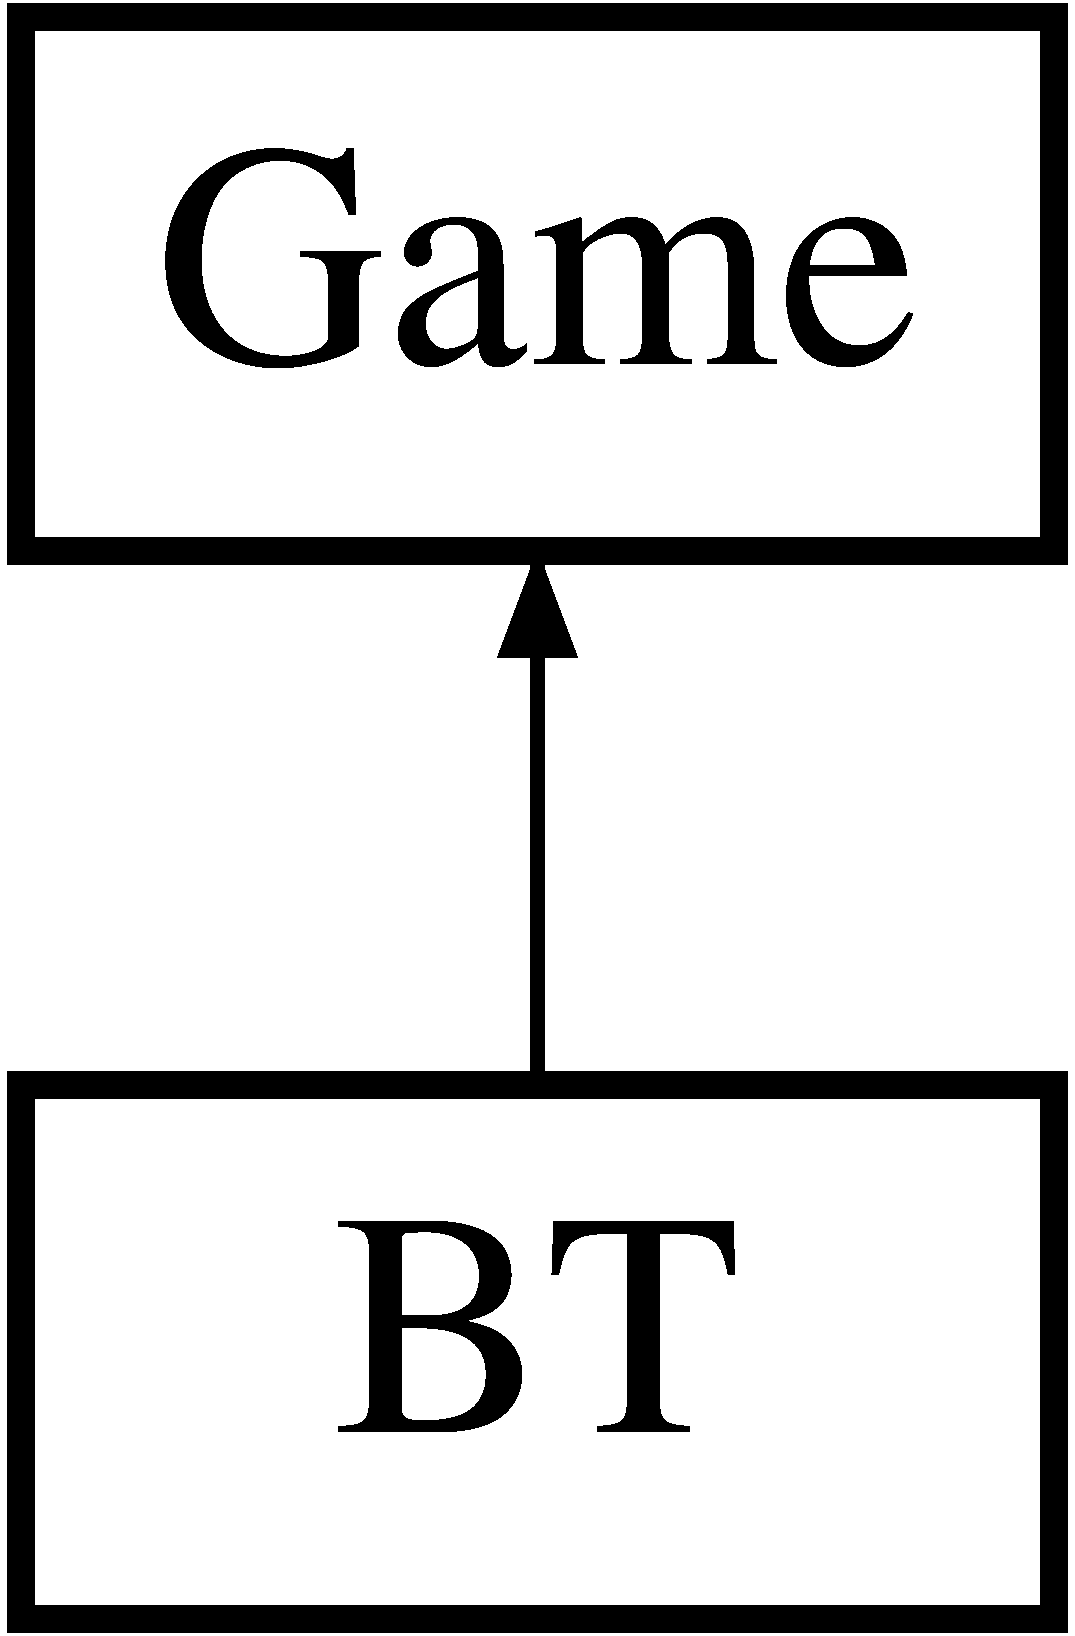
\includegraphics[height=2.000000cm]{class_b_t}
\end{center}
\end{figure}
\subsection*{Public Member Functions}
\begin{DoxyCompactItemize}
\item 
\mbox{\Hypertarget{class_b_t_ace122849e5dcf81df2748b44bec34f97}\label{class_b_t_ace122849e5dcf81df2748b44bec34f97}} 
{\bfseries BT} (int rows, int cols=0)
\item 
virtual std\+::vector$<$ std\+::pair$<$ \hyperlink{class_piece}{Piece}, \hyperlink{class_piece}{Piece} $>$ $>$ \hyperlink{class_b_t_a4d3ad59ecb429b37c983986cc7802b17}{legal\+\_\+moves} ()
\begin{DoxyCompactList}\small\item\em abstract function to check if a move is legal \end{DoxyCompactList}\item 
virtual void \hyperlink{class_b_t_acb87d577e00a5fa66ddb653c697e3ad4}{start} ()
\begin{DoxyCompactList}\small\item\em starts a new instance of the game being played \end{DoxyCompactList}\item 
virtual int \hyperlink{class_b_t_a330840afc9271716265fb65eb037d351}{evaluate} ()
\begin{DoxyCompactList}\small\item\em evaluates the current state of the board \end{DoxyCompactList}\item 
virtual char \hyperlink{class_b_t_a5b09c0eb2d583ae2141aeefe18545e5c}{terminal\+\_\+state} ()
\begin{DoxyCompactList}\small\item\em checks to see if the game has hit a terminal state \end{DoxyCompactList}\end{DoxyCompactItemize}
\subsection*{Additional Inherited Members}


\subsection{Member Function Documentation}
\mbox{\Hypertarget{class_b_t_a330840afc9271716265fb65eb037d351}\label{class_b_t_a330840afc9271716265fb65eb037d351}} 
\index{BT@{BT}!evaluate@{evaluate}}
\index{evaluate@{evaluate}!BT@{BT}}
\subsubsection{\texorpdfstring{evaluate()}{evaluate()}}
{\footnotesize\ttfamily int B\+T\+::evaluate (\begin{DoxyParamCaption}{ }\end{DoxyParamCaption})\hspace{0.3cm}{\ttfamily [virtual]}}



evaluates the current state of the board 

\begin{DoxyReturn}{Returns}
the state evaluation as an integer 
\end{DoxyReturn}


Implements \hyperlink{class_game_a068b2b3012154457f362c90a80f46253}{Game}.

\mbox{\Hypertarget{class_b_t_a4d3ad59ecb429b37c983986cc7802b17}\label{class_b_t_a4d3ad59ecb429b37c983986cc7802b17}} 
\index{BT@{BT}!legal\+\_\+moves@{legal\+\_\+moves}}
\index{legal\+\_\+moves@{legal\+\_\+moves}!BT@{BT}}
\subsubsection{\texorpdfstring{legal\+\_\+moves()}{legal\_moves()}}
{\footnotesize\ttfamily vector$<$ pair$<$ \hyperlink{class_piece}{Piece}, \hyperlink{class_piece}{Piece} $>$ $>$ B\+T\+::legal\+\_\+moves (\begin{DoxyParamCaption}{ }\end{DoxyParamCaption})\hspace{0.3cm}{\ttfamily [virtual]}}



abstract function to check if a move is legal 

\begin{DoxyReturn}{Returns}
a vector of legal moves for the player whos turn it is 
\end{DoxyReturn}


Implements \hyperlink{class_game_a205fc7dd195bc398138cc188aad8bc38}{Game}.

\mbox{\Hypertarget{class_b_t_acb87d577e00a5fa66ddb653c697e3ad4}\label{class_b_t_acb87d577e00a5fa66ddb653c697e3ad4}} 
\index{BT@{BT}!start@{start}}
\index{start@{start}!BT@{BT}}
\subsubsection{\texorpdfstring{start()}{start()}}
{\footnotesize\ttfamily void B\+T\+::start (\begin{DoxyParamCaption}{ }\end{DoxyParamCaption})\hspace{0.3cm}{\ttfamily [virtual]}}



starts a new instance of the game being played 



Implements \hyperlink{class_game_add988158041df85337995e36f06756aa}{Game}.

\mbox{\Hypertarget{class_b_t_a5b09c0eb2d583ae2141aeefe18545e5c}\label{class_b_t_a5b09c0eb2d583ae2141aeefe18545e5c}} 
\index{BT@{BT}!terminal\+\_\+state@{terminal\+\_\+state}}
\index{terminal\+\_\+state@{terminal\+\_\+state}!BT@{BT}}
\subsubsection{\texorpdfstring{terminal\+\_\+state()}{terminal\_state()}}
{\footnotesize\ttfamily char B\+T\+::terminal\+\_\+state (\begin{DoxyParamCaption}{ }\end{DoxyParamCaption})\hspace{0.3cm}{\ttfamily [virtual]}}



checks to see if the game has hit a terminal state 

\begin{DoxyReturn}{Returns}
a character value to represent the state of the game 
\end{DoxyReturn}


Implements \hyperlink{class_game_ac7cbe36964272dd7dcd7e68fafaf24cc}{Game}.



The documentation for this class was generated from the following files\+:\begin{DoxyCompactItemize}
\item 
B\+T.\+h\item 
B\+T.\+cpp\end{DoxyCompactItemize}

\hypertarget{class_fa_h}{}\section{FaH Class Reference}
\label{class_fa_h}\index{FaH@{FaH}}
Inheritance diagram for FaH\+:\begin{figure}[H]
\begin{center}
\leavevmode
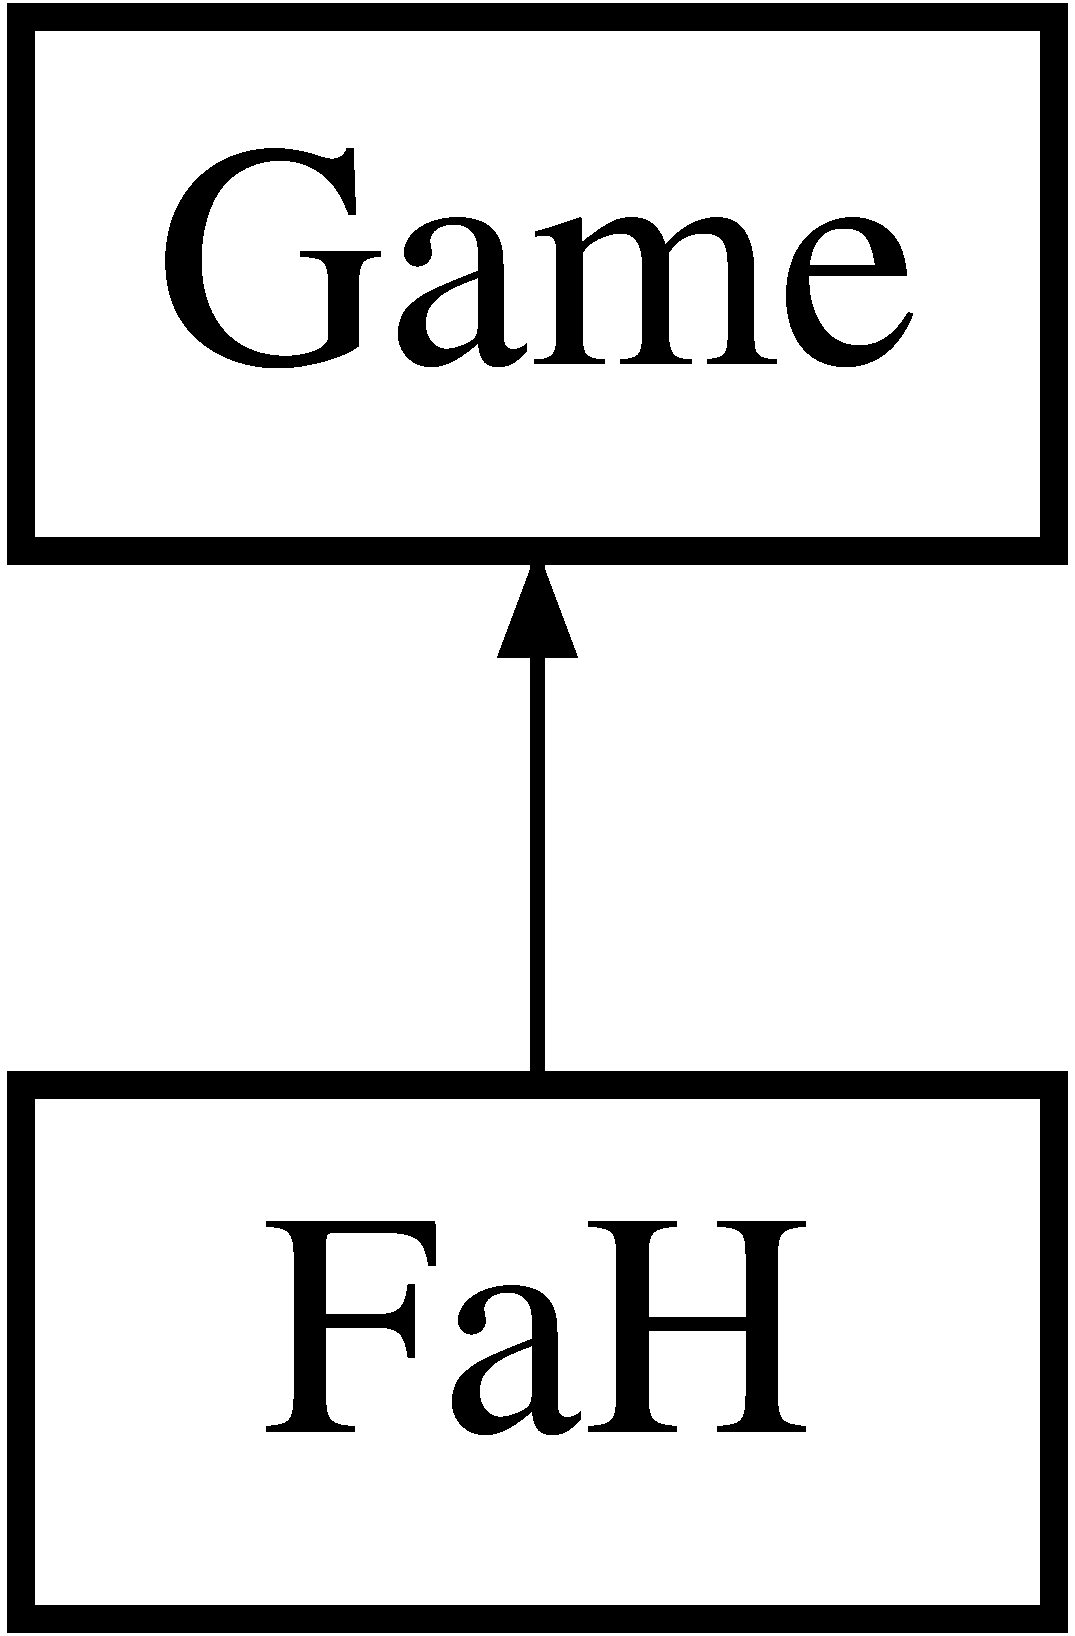
\includegraphics[height=2.000000cm]{class_fa_h}
\end{center}
\end{figure}
\subsection*{Public Member Functions}
\begin{DoxyCompactItemize}
\item 
\mbox{\Hypertarget{class_fa_h_a6bf4d1735a23a2cf51cfe905c4f437a8}\label{class_fa_h_a6bf4d1735a23a2cf51cfe905c4f437a8}} 
virtual std\+::vector$<$ std\+::pair$<$ \hyperlink{class_piece}{Piece}, \hyperlink{class_piece}{Piece} $>$ $>$ {\bfseries legal\+\_\+moves} ()
\item 
\mbox{\Hypertarget{class_fa_h_a79788a0309788fed655c77bea2167110}\label{class_fa_h_a79788a0309788fed655c77bea2167110}} 
virtual int {\bfseries evaluate} ()
\item 
\mbox{\Hypertarget{class_fa_h_a21c22430a8fa6d3654cb29244d04d0ab}\label{class_fa_h_a21c22430a8fa6d3654cb29244d04d0ab}} 
virtual void {\bfseries start} ()
\item 
\mbox{\Hypertarget{class_fa_h_a575223df37dc4b747634a7873e399275}\label{class_fa_h_a575223df37dc4b747634a7873e399275}} 
virtual char {\bfseries terminal\+\_\+state} ()
\end{DoxyCompactItemize}
\subsection*{Additional Inherited Members}


The documentation for this class was generated from the following files\+:\begin{DoxyCompactItemize}
\item 
Fa\+H.\+h\item 
Fa\+H.\+cpp\end{DoxyCompactItemize}

\hypertarget{class_game}{}\section{Game Class Reference}
\label{class_game}\index{Game@{Game}}
Inheritance diagram for Game\+:\begin{figure}[H]
\begin{center}
\leavevmode
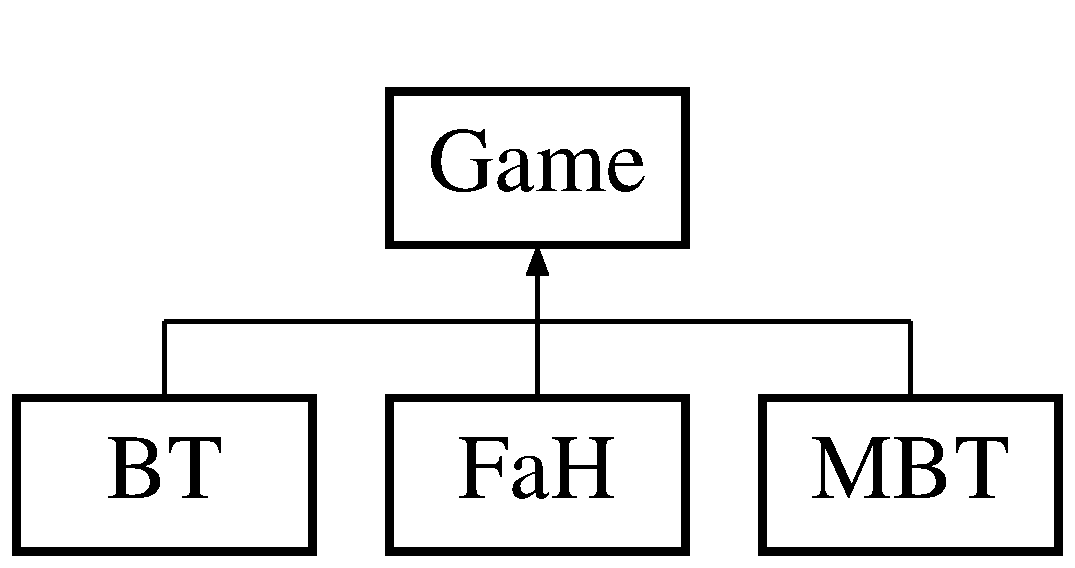
\includegraphics[height=2.000000cm]{class_game}
\end{center}
\end{figure}
\subsection*{Public Member Functions}
\begin{DoxyCompactItemize}
\item 
\hyperlink{class_game_ac8c9003009977a0ecf0c35e0002f0f9e}{Game} (int rows, int cols=0)
\begin{DoxyCompactList}\small\item\em initializes the size of the board \end{DoxyCompactList}\item 
virtual std\+::vector$<$ std\+::pair$<$ \hyperlink{class_piece}{Piece}, \hyperlink{class_piece}{Piece} $>$ $>$ \hyperlink{class_game_a205fc7dd195bc398138cc188aad8bc38}{legal\+\_\+moves} ()=0
\begin{DoxyCompactList}\small\item\em abstract function to check if a move is legal \end{DoxyCompactList}\item 
virtual void \hyperlink{class_game_add988158041df85337995e36f06756aa}{start} ()=0
\begin{DoxyCompactList}\small\item\em starts a new instance of the game being played \end{DoxyCompactList}\item 
virtual int \hyperlink{class_game_a068b2b3012154457f362c90a80f46253}{evaluate} ()=0
\begin{DoxyCompactList}\small\item\em evaluates the current state of the board \end{DoxyCompactList}\item 
virtual char \hyperlink{class_game_ac7cbe36964272dd7dcd7e68fafaf24cc}{terminal\+\_\+state} ()=0
\begin{DoxyCompactList}\small\item\em checks to see if the game has hit a terminal state \end{DoxyCompactList}\item 
\mbox{\Hypertarget{class_game_a69f0e2636aa7e85836418aea42792527}\label{class_game_a69f0e2636aa7e85836418aea42792527}} 
void \hyperlink{class_game_a69f0e2636aa7e85836418aea42792527}{legal} ()
\begin{DoxyCompactList}\small\item\em uses legel\+\_\+moves() to find all legal moves for the player whos turn it is \end{DoxyCompactList}\item 
void \hyperlink{class_game_ae98bb6563800f3265d7da2445804ea97}{display} () const
\begin{DoxyCompactList}\small\item\em displays the current game board and info to the console \end{DoxyCompactList}\item 
void \hyperlink{class_game_a00150c33b3469c2fb95653b2f3be36b6}{move} (std\+::string from, std\+::string to)
\begin{DoxyCompactList}\small\item\em moves a piece \end{DoxyCompactList}\item 
void \hyperlink{class_game_a9be0655102af94f1a37a7eaec1be36fc}{retract} ()
\begin{DoxyCompactList}\small\item\em moves the game one turn back in time \end{DoxyCompactList}\item 
void \hyperlink{class_game_accc03cc11af1ef5614a265d2e9ed4841}{record\+\_\+time} ()
\begin{DoxyCompactList}\small\item\em saves the game so it can be called with \hyperlink{class_game_a9be0655102af94f1a37a7eaec1be36fc}{retract()} \end{DoxyCompactList}\item 
\hyperlink{struct_position}{Position} \hyperlink{class_game_a2a71f9781d47c4b7c62005bb14f6bfa3}{get\+\_\+int\+\_\+from\+\_\+input} (std\+::string input)
\begin{DoxyCompactList}\small\item\em returns integer value for a string \end{DoxyCompactList}\item 
\hyperlink{class_piece}{Piece} \hyperlink{class_game_a255e5bb1512854fd8df8cef51fab49d8}{get\+\_\+at\+\_\+board} (int x, int y)
\begin{DoxyCompactList}\small\item\em find a \hyperlink{class_piece}{Piece} with specific coordinates \end{DoxyCompactList}\item 
void \hyperlink{class_game_ac495c211545773a11948a3b3ac52bb18}{A\+I\+\_\+move} ()
\begin{DoxyCompactList}\small\item\em Lets the AI move for the player whos turn it is depending on the difficulty. \end{DoxyCompactList}\item 
\mbox{\Hypertarget{class_game_aed72a88415e4978d27c72e6929264e0d}\label{class_game_aed72a88415e4978d27c72e6929264e0d}} 
void {\bfseries set\+\_\+level} (char l)
\item 
\mbox{\Hypertarget{class_game_a0643486d59cd27c1089d97ecffec1c79}\label{class_game_a0643486d59cd27c1089d97ecffec1c79}} 
char {\bfseries get\+\_\+level} ()
\item 
\mbox{\Hypertarget{class_game_a65250bbb867f1eb8067dab620a1dfd58}\label{class_game_a65250bbb867f1eb8067dab620a1dfd58}} 
int {\bfseries get\+\_\+turns} ()
\end{DoxyCompactItemize}
\subsection*{Protected Attributes}
\begin{DoxyCompactItemize}
\item 
\mbox{\Hypertarget{class_game_ade066636bda0bcc3501deb4981d9f400}\label{class_game_ade066636bda0bcc3501deb4981d9f400}} 
\hyperlink{class_board}{Board} $\ast$ {\bfseries board\+\_\+}
\item 
\mbox{\Hypertarget{class_game_abc9f7b7f1ced3ddb136dbd25bebd4e2a}\label{class_game_abc9f7b7f1ced3ddb136dbd25bebd4e2a}} 
int {\bfseries turn\+\_\+}
\item 
\mbox{\Hypertarget{class_game_aacf1e01c0a9777117e730c8105fc339c}\label{class_game_aacf1e01c0a9777117e730c8105fc339c}} 
std\+::vector$<$ \hyperlink{class_board}{Board} $\ast$ $>$ {\bfseries timeline\+\_\+}
\item 
\mbox{\Hypertarget{class_game_a9fcfb58bda101e497f8845f01ba56582}\label{class_game_a9fcfb58bda101e497f8845f01ba56582}} 
char {\bfseries level\+\_\+}
\end{DoxyCompactItemize}


\subsection{Constructor \& Destructor Documentation}
\mbox{\Hypertarget{class_game_ac8c9003009977a0ecf0c35e0002f0f9e}\label{class_game_ac8c9003009977a0ecf0c35e0002f0f9e}} 
\index{Game@{Game}!Game@{Game}}
\index{Game@{Game}!Game@{Game}}
\subsubsection{\texorpdfstring{Game()}{Game()}}
{\footnotesize\ttfamily Game\+::\+Game (\begin{DoxyParamCaption}\item[{int}]{rows,  }\item[{int}]{cols = {\ttfamily 0} }\end{DoxyParamCaption})}



initializes the size of the board 


\begin{DoxyParams}{Parameters}
{\em rows} & for number of rows \\
\hline
{\em cols} & for number of columns \\
\hline
\end{DoxyParams}


\subsection{Member Function Documentation}
\mbox{\Hypertarget{class_game_ac495c211545773a11948a3b3ac52bb18}\label{class_game_ac495c211545773a11948a3b3ac52bb18}} 
\index{Game@{Game}!A\+I\+\_\+move@{A\+I\+\_\+move}}
\index{A\+I\+\_\+move@{A\+I\+\_\+move}!Game@{Game}}
\subsubsection{\texorpdfstring{A\+I\+\_\+move()}{AI\_move()}}
{\footnotesize\ttfamily void Game\+::\+A\+I\+\_\+move (\begin{DoxyParamCaption}{ }\end{DoxyParamCaption})}



Lets the AI move for the player whos turn it is depending on the difficulty. 

\mbox{\Hypertarget{class_game_ae98bb6563800f3265d7da2445804ea97}\label{class_game_ae98bb6563800f3265d7da2445804ea97}} 
\index{Game@{Game}!display@{display}}
\index{display@{display}!Game@{Game}}
\subsubsection{\texorpdfstring{display()}{display()}}
{\footnotesize\ttfamily void Game\+::display (\begin{DoxyParamCaption}{ }\end{DoxyParamCaption}) const}



displays the current game board and info to the console 

\mbox{\Hypertarget{class_game_a068b2b3012154457f362c90a80f46253}\label{class_game_a068b2b3012154457f362c90a80f46253}} 
\index{Game@{Game}!evaluate@{evaluate}}
\index{evaluate@{evaluate}!Game@{Game}}
\subsubsection{\texorpdfstring{evaluate()}{evaluate()}}
{\footnotesize\ttfamily virtual int Game\+::evaluate (\begin{DoxyParamCaption}{ }\end{DoxyParamCaption})\hspace{0.3cm}{\ttfamily [pure virtual]}}



evaluates the current state of the board 

\begin{DoxyReturn}{Returns}
the state evaluation as an integer 
\end{DoxyReturn}


Implemented in \hyperlink{class_b_t_a330840afc9271716265fb65eb037d351}{BT}, \hyperlink{class_m_b_t_a62bfe73fc6dd6da20650f27024dd0115}{M\+BT}, and \hyperlink{class_fa_h_a79788a0309788fed655c77bea2167110}{FaH}.

\mbox{\Hypertarget{class_game_a255e5bb1512854fd8df8cef51fab49d8}\label{class_game_a255e5bb1512854fd8df8cef51fab49d8}} 
\index{Game@{Game}!get\+\_\+at\+\_\+board@{get\+\_\+at\+\_\+board}}
\index{get\+\_\+at\+\_\+board@{get\+\_\+at\+\_\+board}!Game@{Game}}
\subsubsection{\texorpdfstring{get\+\_\+at\+\_\+board()}{get\_at\_board()}}
{\footnotesize\ttfamily \hyperlink{class_piece}{Piece} Game\+::get\+\_\+at\+\_\+board (\begin{DoxyParamCaption}\item[{int}]{x,  }\item[{int}]{y }\end{DoxyParamCaption})}



find a \hyperlink{class_piece}{Piece} with specific coordinates 


\begin{DoxyParams}{Parameters}
{\em x} & coord \\
\hline
{\em y} & coord \\
\hline
\end{DoxyParams}
\begin{DoxyReturn}{Returns}
\hyperlink{class_piece}{Piece} with given coordinate 
\end{DoxyReturn}
\mbox{\Hypertarget{class_game_a2a71f9781d47c4b7c62005bb14f6bfa3}\label{class_game_a2a71f9781d47c4b7c62005bb14f6bfa3}} 
\index{Game@{Game}!get\+\_\+int\+\_\+from\+\_\+input@{get\+\_\+int\+\_\+from\+\_\+input}}
\index{get\+\_\+int\+\_\+from\+\_\+input@{get\+\_\+int\+\_\+from\+\_\+input}!Game@{Game}}
\subsubsection{\texorpdfstring{get\+\_\+int\+\_\+from\+\_\+input()}{get\_int\_from\_input()}}
{\footnotesize\ttfamily \hyperlink{struct_position}{Position} Game\+::get\+\_\+int\+\_\+from\+\_\+input (\begin{DoxyParamCaption}\item[{std\+::string}]{input }\end{DoxyParamCaption})}



returns integer value for a string 


\begin{DoxyParams}{Parameters}
{\em input} & square name e.\+g. a1 \\
\hline
\end{DoxyParams}
\mbox{\Hypertarget{class_game_a205fc7dd195bc398138cc188aad8bc38}\label{class_game_a205fc7dd195bc398138cc188aad8bc38}} 
\index{Game@{Game}!legal\+\_\+moves@{legal\+\_\+moves}}
\index{legal\+\_\+moves@{legal\+\_\+moves}!Game@{Game}}
\subsubsection{\texorpdfstring{legal\+\_\+moves()}{legal\_moves()}}
{\footnotesize\ttfamily virtual std\+::vector$<$std\+::pair$<$\hyperlink{class_piece}{Piece},\hyperlink{class_piece}{Piece}$>$ $>$ Game\+::legal\+\_\+moves (\begin{DoxyParamCaption}{ }\end{DoxyParamCaption})\hspace{0.3cm}{\ttfamily [pure virtual]}}



abstract function to check if a move is legal 

\begin{DoxyReturn}{Returns}
a vector of legal moves for the player whos turn it is 
\end{DoxyReturn}


Implemented in \hyperlink{class_b_t_a4d3ad59ecb429b37c983986cc7802b17}{BT}, \hyperlink{class_m_b_t_add9f32f140d4c6fb5e160eadeddd6738}{M\+BT}, and \hyperlink{class_fa_h_a6bf4d1735a23a2cf51cfe905c4f437a8}{FaH}.

\mbox{\Hypertarget{class_game_a00150c33b3469c2fb95653b2f3be36b6}\label{class_game_a00150c33b3469c2fb95653b2f3be36b6}} 
\index{Game@{Game}!move@{move}}
\index{move@{move}!Game@{Game}}
\subsubsection{\texorpdfstring{move()}{move()}}
{\footnotesize\ttfamily void Game\+::move (\begin{DoxyParamCaption}\item[{std\+::string}]{from,  }\item[{std\+::string}]{to }\end{DoxyParamCaption})}



moves a piece 


\begin{DoxyParams}{Parameters}
{\em from} & \+: start position \\
\hline
{\em to} & \+: end position \\
\hline
\end{DoxyParams}
\mbox{\Hypertarget{class_game_accc03cc11af1ef5614a265d2e9ed4841}\label{class_game_accc03cc11af1ef5614a265d2e9ed4841}} 
\index{Game@{Game}!record\+\_\+time@{record\+\_\+time}}
\index{record\+\_\+time@{record\+\_\+time}!Game@{Game}}
\subsubsection{\texorpdfstring{record\+\_\+time()}{record\_time()}}
{\footnotesize\ttfamily void Game\+::record\+\_\+time (\begin{DoxyParamCaption}{ }\end{DoxyParamCaption})}



saves the game so it can be called with \hyperlink{class_game_a9be0655102af94f1a37a7eaec1be36fc}{retract()} 

\mbox{\Hypertarget{class_game_a9be0655102af94f1a37a7eaec1be36fc}\label{class_game_a9be0655102af94f1a37a7eaec1be36fc}} 
\index{Game@{Game}!retract@{retract}}
\index{retract@{retract}!Game@{Game}}
\subsubsection{\texorpdfstring{retract()}{retract()}}
{\footnotesize\ttfamily void Game\+::retract (\begin{DoxyParamCaption}{ }\end{DoxyParamCaption})}



moves the game one turn back in time 

\mbox{\Hypertarget{class_game_add988158041df85337995e36f06756aa}\label{class_game_add988158041df85337995e36f06756aa}} 
\index{Game@{Game}!start@{start}}
\index{start@{start}!Game@{Game}}
\subsubsection{\texorpdfstring{start()}{start()}}
{\footnotesize\ttfamily virtual void Game\+::start (\begin{DoxyParamCaption}{ }\end{DoxyParamCaption})\hspace{0.3cm}{\ttfamily [pure virtual]}}



starts a new instance of the game being played 



Implemented in \hyperlink{class_b_t_acb87d577e00a5fa66ddb653c697e3ad4}{BT}, \hyperlink{class_fa_h_a21c22430a8fa6d3654cb29244d04d0ab}{FaH}, and \hyperlink{class_m_b_t_aa951382dfec95e214ba1e63189977d8f}{M\+BT}.

\mbox{\Hypertarget{class_game_ac7cbe36964272dd7dcd7e68fafaf24cc}\label{class_game_ac7cbe36964272dd7dcd7e68fafaf24cc}} 
\index{Game@{Game}!terminal\+\_\+state@{terminal\+\_\+state}}
\index{terminal\+\_\+state@{terminal\+\_\+state}!Game@{Game}}
\subsubsection{\texorpdfstring{terminal\+\_\+state()}{terminal\_state()}}
{\footnotesize\ttfamily virtual char Game\+::terminal\+\_\+state (\begin{DoxyParamCaption}{ }\end{DoxyParamCaption})\hspace{0.3cm}{\ttfamily [pure virtual]}}



checks to see if the game has hit a terminal state 

\begin{DoxyReturn}{Returns}
a character value to represent the state of the game 
\end{DoxyReturn}


Implemented in \hyperlink{class_b_t_a5b09c0eb2d583ae2141aeefe18545e5c}{BT}, \hyperlink{class_m_b_t_ac0b5fc7a538c643ce69a678407fa9f56}{M\+BT}, and \hyperlink{class_fa_h_a575223df37dc4b747634a7873e399275}{FaH}.



The documentation for this class was generated from the following files\+:\begin{DoxyCompactItemize}
\item 
Game.\+h\item 
Game.\+cpp\end{DoxyCompactItemize}

\hypertarget{class_m_b_t}{}\section{M\+BT Class Reference}
\label{class_m_b_t}\index{M\+BT@{M\+BT}}
Inheritance diagram for M\+BT\+:\begin{figure}[H]
\begin{center}
\leavevmode
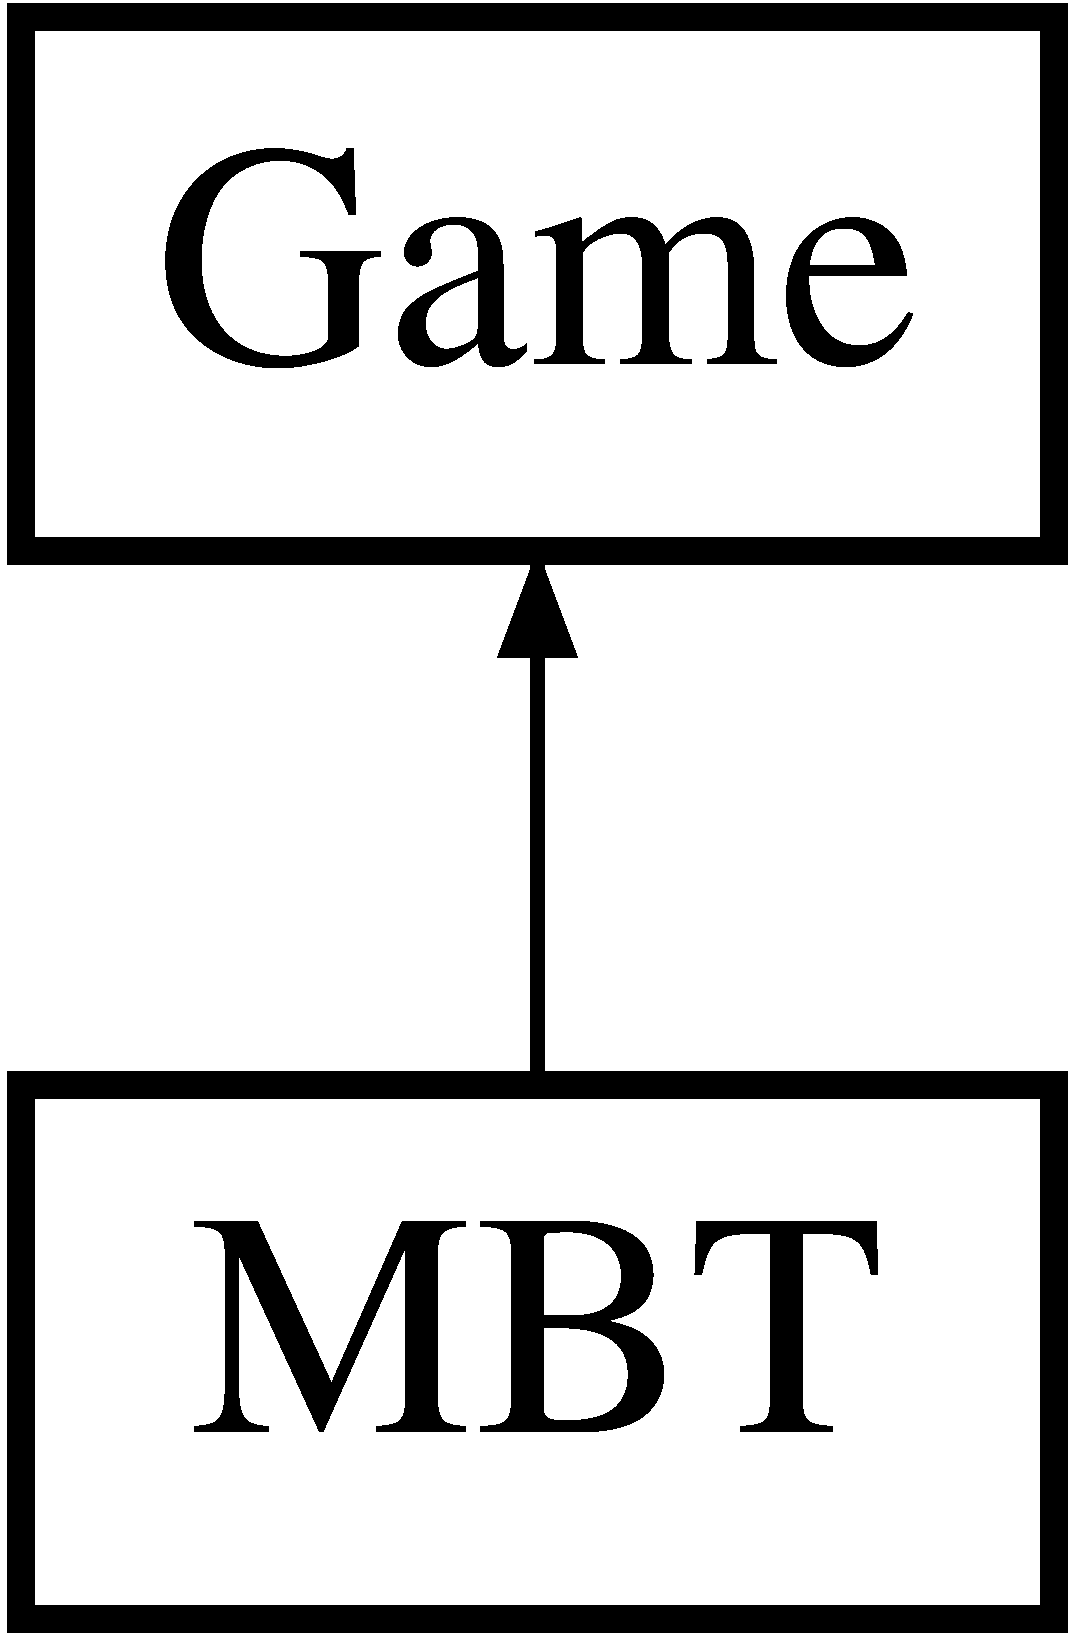
\includegraphics[height=2.000000cm]{class_m_b_t}
\end{center}
\end{figure}
\subsection*{Public Member Functions}
\begin{DoxyCompactItemize}
\item 
\mbox{\Hypertarget{class_m_b_t_a443c36b0b0281555ead87d21ff92082a}\label{class_m_b_t_a443c36b0b0281555ead87d21ff92082a}} 
{\bfseries M\+BT} (int rows, int cols=0)
\item 
virtual std\+::vector$<$ std\+::pair$<$ \hyperlink{class_piece}{Piece}, \hyperlink{class_piece}{Piece} $>$ $>$ \hyperlink{class_m_b_t_add9f32f140d4c6fb5e160eadeddd6738}{legal\+\_\+moves} ()
\begin{DoxyCompactList}\small\item\em abstract function to check if a move is legal \end{DoxyCompactList}\item 
virtual void \hyperlink{class_m_b_t_aa951382dfec95e214ba1e63189977d8f}{start} ()
\begin{DoxyCompactList}\small\item\em starts a new instance of the game being played \end{DoxyCompactList}\item 
virtual int \hyperlink{class_m_b_t_a62bfe73fc6dd6da20650f27024dd0115}{evaluate} ()
\begin{DoxyCompactList}\small\item\em evaluates the current state of the board \end{DoxyCompactList}\item 
virtual char \hyperlink{class_m_b_t_ac0b5fc7a538c643ce69a678407fa9f56}{terminal\+\_\+state} ()
\begin{DoxyCompactList}\small\item\em checks to see if the game has hit a terminal state \end{DoxyCompactList}\end{DoxyCompactItemize}
\subsection*{Additional Inherited Members}


\subsection{Member Function Documentation}
\mbox{\Hypertarget{class_m_b_t_a62bfe73fc6dd6da20650f27024dd0115}\label{class_m_b_t_a62bfe73fc6dd6da20650f27024dd0115}} 
\index{M\+BT@{M\+BT}!evaluate@{evaluate}}
\index{evaluate@{evaluate}!M\+BT@{M\+BT}}
\subsubsection{\texorpdfstring{evaluate()}{evaluate()}}
{\footnotesize\ttfamily int M\+B\+T\+::evaluate (\begin{DoxyParamCaption}{ }\end{DoxyParamCaption})\hspace{0.3cm}{\ttfamily [virtual]}}



evaluates the current state of the board 

\begin{DoxyReturn}{Returns}
the state evaluation as an integer 
\end{DoxyReturn}


Implements \hyperlink{class_game_a068b2b3012154457f362c90a80f46253}{Game}.

\mbox{\Hypertarget{class_m_b_t_add9f32f140d4c6fb5e160eadeddd6738}\label{class_m_b_t_add9f32f140d4c6fb5e160eadeddd6738}} 
\index{M\+BT@{M\+BT}!legal\+\_\+moves@{legal\+\_\+moves}}
\index{legal\+\_\+moves@{legal\+\_\+moves}!M\+BT@{M\+BT}}
\subsubsection{\texorpdfstring{legal\+\_\+moves()}{legal\_moves()}}
{\footnotesize\ttfamily std\+::vector$<$ std\+::pair$<$ \hyperlink{class_piece}{Piece}, \hyperlink{class_piece}{Piece} $>$ $>$ M\+B\+T\+::legal\+\_\+moves (\begin{DoxyParamCaption}{ }\end{DoxyParamCaption})\hspace{0.3cm}{\ttfamily [virtual]}}



abstract function to check if a move is legal 

\begin{DoxyReturn}{Returns}
a vector of legal moves for the player whos turn it is 
\end{DoxyReturn}


Implements \hyperlink{class_game_a205fc7dd195bc398138cc188aad8bc38}{Game}.

\mbox{\Hypertarget{class_m_b_t_aa951382dfec95e214ba1e63189977d8f}\label{class_m_b_t_aa951382dfec95e214ba1e63189977d8f}} 
\index{M\+BT@{M\+BT}!start@{start}}
\index{start@{start}!M\+BT@{M\+BT}}
\subsubsection{\texorpdfstring{start()}{start()}}
{\footnotesize\ttfamily void M\+B\+T\+::start (\begin{DoxyParamCaption}{ }\end{DoxyParamCaption})\hspace{0.3cm}{\ttfamily [virtual]}}



starts a new instance of the game being played 



Implements \hyperlink{class_game_add988158041df85337995e36f06756aa}{Game}.

\mbox{\Hypertarget{class_m_b_t_ac0b5fc7a538c643ce69a678407fa9f56}\label{class_m_b_t_ac0b5fc7a538c643ce69a678407fa9f56}} 
\index{M\+BT@{M\+BT}!terminal\+\_\+state@{terminal\+\_\+state}}
\index{terminal\+\_\+state@{terminal\+\_\+state}!M\+BT@{M\+BT}}
\subsubsection{\texorpdfstring{terminal\+\_\+state()}{terminal\_state()}}
{\footnotesize\ttfamily char M\+B\+T\+::terminal\+\_\+state (\begin{DoxyParamCaption}{ }\end{DoxyParamCaption})\hspace{0.3cm}{\ttfamily [virtual]}}



checks to see if the game has hit a terminal state 

\begin{DoxyReturn}{Returns}
a character value to represent the state of the game 
\end{DoxyReturn}


Implements \hyperlink{class_game_ac7cbe36964272dd7dcd7e68fafaf24cc}{Game}.



The documentation for this class was generated from the following files\+:\begin{DoxyCompactItemize}
\item 
M\+B\+T.\+h\item 
M\+B\+T.\+cpp\end{DoxyCompactItemize}

\hypertarget{class_piece}{}\section{Piece Class Reference}
\label{class_piece}\index{Piece@{Piece}}
\subsection*{Public Member Functions}
\begin{DoxyCompactItemize}
\item 
\mbox{\Hypertarget{class_piece_af1d9eb7f67a06fd1dec6c990c95b5801}\label{class_piece_af1d9eb7f67a06fd1dec6c990c95b5801}} 
{\bfseries Piece} (int x, int y)
\item 
\mbox{\Hypertarget{class_piece_a14670dac899c8c3ea9efe5e11a87fd85}\label{class_piece_a14670dac899c8c3ea9efe5e11a87fd85}} 
{\bfseries Piece} (int player, char sym, \hyperlink{struct_position}{Position} pos, std\+::vector$<$ std\+::pair$<$ int, int $>$$>$ moves)
\item 
\mbox{\Hypertarget{class_piece_ad0eb90d1f75a909240d98ed70d72e4f4}\label{class_piece_ad0eb90d1f75a909240d98ed70d72e4f4}} 
char {\bfseries get\+\_\+symbol} () const
\item 
\mbox{\Hypertarget{class_piece_ab588439a98647b6b6deef620be16e7ae}\label{class_piece_ab588439a98647b6b6deef620be16e7ae}} 
int {\bfseries get\+\_\+owner} () const
\item 
\mbox{\Hypertarget{class_piece_a6dcc7df628eb1f8317caaa4970835517}\label{class_piece_a6dcc7df628eb1f8317caaa4970835517}} 
\hyperlink{struct_position}{Position} {\bfseries get\+\_\+position} () const
\item 
\mbox{\Hypertarget{class_piece_a20bfbba13742685ede3fbde882f9cbf5}\label{class_piece_a20bfbba13742685ede3fbde882f9cbf5}} 
void {\bfseries set\+\_\+position} (int x, int y)
\item 
\mbox{\Hypertarget{class_piece_a328672e36bcdd76b0ea1892e3a733bda}\label{class_piece_a328672e36bcdd76b0ea1892e3a733bda}} 
std\+::vector$<$ std\+::pair$<$ int, int $>$ $>$ {\bfseries get\+\_\+posible\+\_\+moves} () const
\item 
\mbox{\Hypertarget{class_piece_a874649d960a257b6fa24baa3319fb5e8}\label{class_piece_a874649d960a257b6fa24baa3319fb5e8}} 
bool {\bfseries operator==} (const \hyperlink{class_piece}{Piece} \&rhs) const
\end{DoxyCompactItemize}


The documentation for this class was generated from the following files\+:\begin{DoxyCompactItemize}
\item 
Piece.\+h\item 
Piece.\+cpp\end{DoxyCompactItemize}

\hypertarget{class_player}{}\section{Player Class Reference}
\label{class_player}\index{Player@{Player}}
\subsection*{Public Member Functions}
\begin{DoxyCompactItemize}
\item 
\mbox{\Hypertarget{class_player_adb32329b21de2fca0d7b8caa3e4562ba}\label{class_player_adb32329b21de2fca0d7b8caa3e4562ba}} 
{\bfseries Player} (int player, char sym, int num\+\_\+pieces)
\item 
\mbox{\Hypertarget{class_player_a063ffb27c65cd9e391bdc4024b47c579}\label{class_player_a063ffb27c65cd9e391bdc4024b47c579}} 
char {\bfseries get\+\_\+symbol} ()
\item 
\mbox{\Hypertarget{class_player_a01e4f35c585d5894021ee15363af0b72}\label{class_player_a01e4f35c585d5894021ee15363af0b72}} 
int {\bfseries get\+\_\+player} ()
\end{DoxyCompactItemize}


The documentation for this class was generated from the following file\+:\begin{DoxyCompactItemize}
\item 
Player.\+h\end{DoxyCompactItemize}

\hypertarget{struct_position}{}\section{Position Struct Reference}
\label{struct_position}\index{Position@{Position}}
\subsection*{Public Attributes}
\begin{DoxyCompactItemize}
\item 
\mbox{\Hypertarget{struct_position_a5eee55bf1718fb7c4f296930c38087fe}\label{struct_position_a5eee55bf1718fb7c4f296930c38087fe}} 
int {\bfseries x\+\_\+}
\item 
\mbox{\Hypertarget{struct_position_ac18ebbc60c7d67bb6b30fc1ef82948af}\label{struct_position_ac18ebbc60c7d67bb6b30fc1ef82948af}} 
int {\bfseries y\+\_\+}
\end{DoxyCompactItemize}


The documentation for this struct was generated from the following file\+:\begin{DoxyCompactItemize}
\item 
Piece.\+h\end{DoxyCompactItemize}

%--- End generated contents ---

% Index
\backmatter
\newpage
\phantomsection
\clearemptydoublepage
\addcontentsline{toc}{chapter}{Index}
\printindex

\end{document}
